\documentclass[12pt,letterpaper]{article}
\usepackage[T1]{fontenc}
\usepackage{booktabs}
\usepackage{array} 
\usepackage{latexsym}
\usepackage{amsfonts}
\usepackage{amsmath}
\usepackage{amssymb}
\usepackage{amsthm}
\usepackage{graphicx}
\usepackage[all]{xy}
\usepackage{tikz}
\usepackage[normalem]{ulem}
\usepackage{soul}
\usepackage[utf8]{inputenc}
\usepackage[retainorgcmds]{IEEEtrantools}
\usepackage{upgreek}
\addtolength{\hoffset}{-2cm}
\addtolength{\textwidth}{4cm}
\addtolength{\voffset}{-2.5cm}
\addtolength{\textheight}{5cm}
\pagestyle{empty}
\usepackage{verbatim}
\usepackage{listings}
\usepackage{xcolor}
\usepackage{enumerate}
\usepackage{algorithm2e}
\usepackage{biblatex}
\usepackage{tabularx}
\usepackage{ragged2e}

\newcolumntype{Y}{>{\RaggedRight\arraybackslash}X}
\addbibresource{referencias.bib}

\lstset{
    basicstyle=\ttfamily\small,
    breaklines=true,
    frame=single,
    language=Lisp,
    keywordstyle=\color{blue},
    commentstyle=\color{gray},
    stringstyle=\color{red}
}

\begin{document}

\begin{titlepage}
    
\setlength{\parindent}{0cm}
\rule{\linewidth}{0.1mm}
\begin{center}
    \begin{minipage}{2.5cm}
    	\begin{center}
	    \includegraphics[height=3.4cm]{imagenes/logo_unam.png}
    	\end{center}
    \end{minipage}\hfill
    \begin{minipage}{9.6cm}
    	\begin{center}
    	\textbf{Universidad Nacional Autónoma de México}\\[0.1cm]
        \textbf{Facultad de Ciencias}\\[0.1cm]
        \textbf{Lenguajes de Programación}\\[0.1cm]
        Práctica 5\\[0.1cm]
        Semestre 2026-1\\[0.1cm]
        22 de Octubre de 2025
    	\end{center}
    \end{minipage}\hfill
    \begin{minipage}{3cm}
    	\begin{center}
    	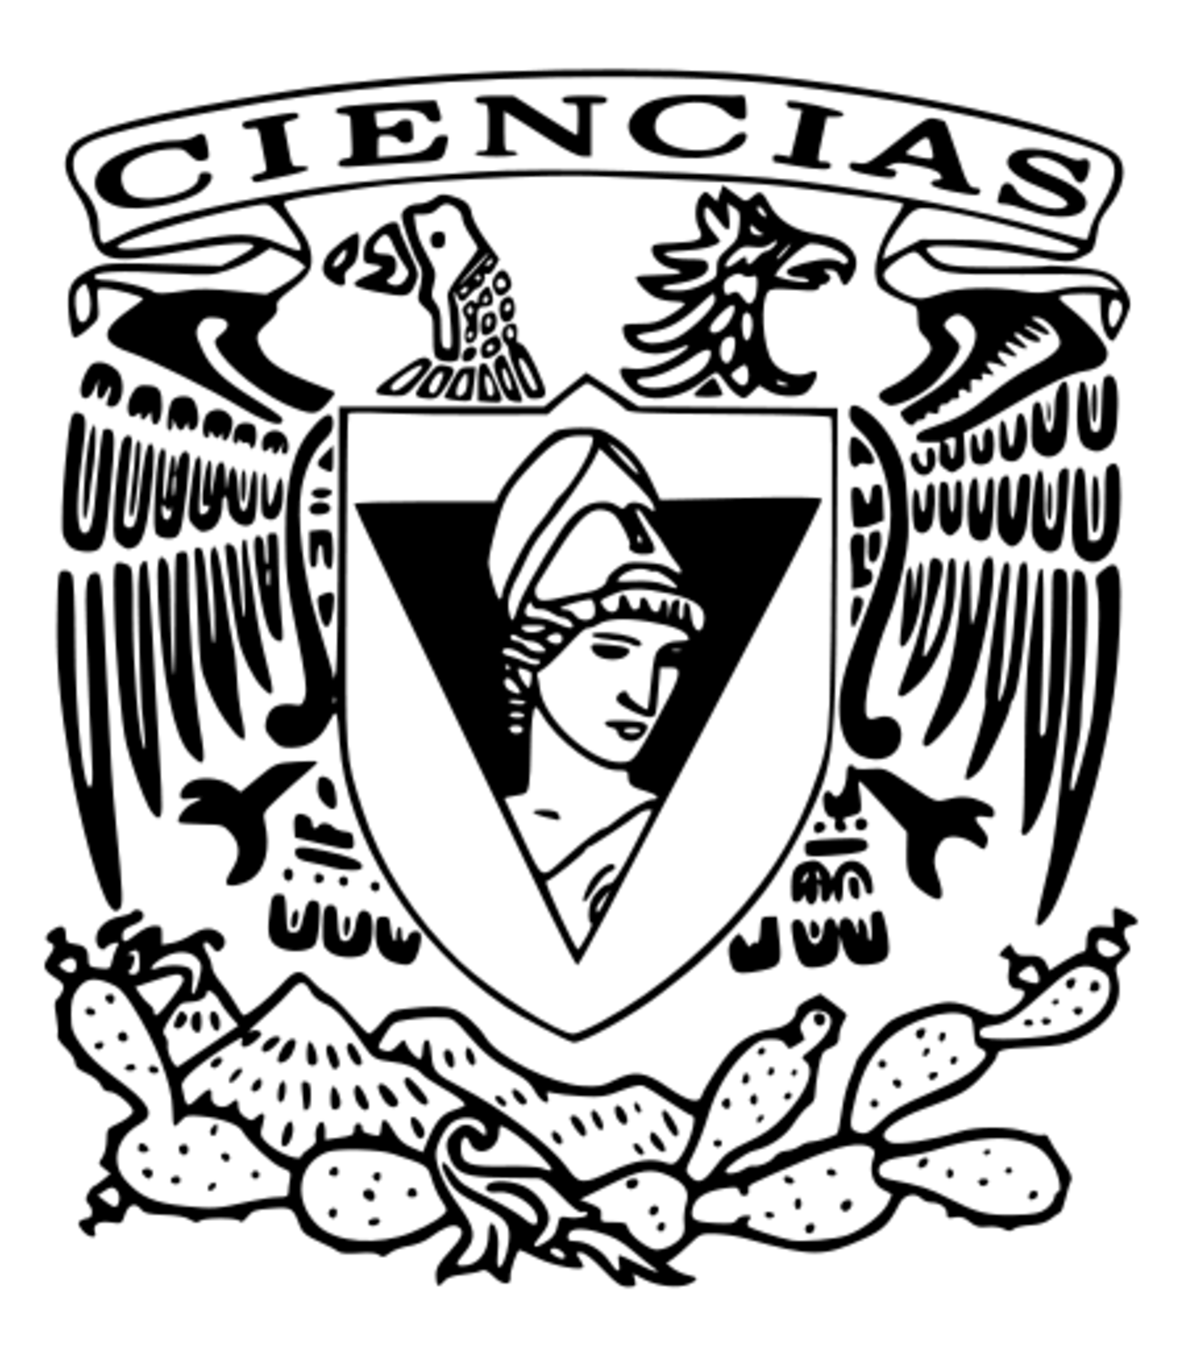
\includegraphics[height=3.6cm]{imagenes/Logo_FC.png}
    	\end{center}
    \end{minipage}
\end{center}

\rule{\linewidth}{0.1mm}\\\\

\textbf{Profesora:}
\begin{itemize}
    \item Dra. Karla Ram\'irez Pulido \\\\
\end{itemize}

\textbf{Ayudantes:}
\begin{itemize}
    \item Alan Alexis Mart\'inez L\'opez \\\\
\end{itemize}

\textbf{Ayudante de laboratorio:}
\begin{itemize}
    \item Karyme Ivette Azpeitia Garc\'ia \\\\
\end{itemize}

\textbf{Integrantes del equipo:}
\begin{itemize}
    \item Gonzalez Castillo Patricio Salvador - 321142391
    \item Valencia Pérez Guillermo Emanuel - 321018689
    \item Rubio Resendiz Marco Antonio - 320209763
    \item Sautto Ramirez Seldon - 321084163
\end{itemize}

\end{titlepage}

\section{Objetivos}

Analizar las implementaciones dadas en los archivos \texttt{grammars.rkt}, \texttt{parser.rkt}, \texttt{desugar.rkt} e \texttt{interp.rkt} para el lenguaje CFWBAE y realizar los siguientes ejercicios.

\subsection{Gramática del lenguaje CFWBAE}

La gramática del lenguaje CFWBAE se presenta a continuación:

\begin{lstlisting}
<expr> ::= <id>
         | <num>
         | <bool>
         | {<op> <expr>+}
         | {if <expr> <expr> <expr>}
         | {cond {<expr> <expr>+} {else <expr>}}
         | {with {{<id> <expr>}+} <expr>}
         | {with* {{<id> <expr>}+} <expr>}
         | {fun {<id>*} <expr>}
         | {<expr> <expr>*}

<id> ::= a | b | c | ...
<num> ::= 1 | 2 | 3 | ...
<bool> ::= true | false
<op> ::= + | - | * | / | modulo | expt | add1 | sub1
       | < | <= | = | > | >= | not | and | or | zero?
\end{lstlisting}

\subsection{Definición de tipos en Racket}

La gramática anterior se define mediante los siguientes tipos en Racket:

\begin{lstlisting}
;; Definicion del tipo Binding
(define-type Binding
  [binding (id symbol?) (value SCFWBAE?)])

;; Definicion del tipo condition para la definicion de cond.
(define-type Condition
  [condition (test-expr SCFWBAE?) (then-expr SCFWBAE?)]
  [else-cond (else-expr SCFWBAE?)])

;; Definicion del tipo SCFWBAE
(define-type SCFWBAE
  [idS (i symbol?)]
  [numS (n number?)]
  [boolS (b boolean?)]
  [iFS (condicion SCFWBAE?) (then SCFWBAE?) (else SCFWBAE?)]
  [opS (f procedure?) (args (listof SCFWBAE?))]
  [condS (cases (listof Condition?))]
  [withS (bindings (listof binding?)) (body SCFWBAE?)]
  [withS* (bindings (listof binding?)) (body SCFWBAE?)]
  [funS (params (listof symbol?)) (body SCFWBAE?)]
  [appS (fun SCFWBAE?) (args (listof SCFWBAE?))])
\end{lstlisting}

\newpage

\section{Ejercicios}

\subsection{Parser}

\begin{enumerate}

\item \textbf{(0.5 pts.) ¿Por qué es importante representar el programa como un árbol de sintaxis abstracta?}


\item \textbf{(1 pts.) Explica cómo el parser reconoce una expresión \texttt{if} y la diferencia respecto al antiguo \texttt{if0}.}

\item \textbf{(0.5 pts.) De acuerdo a la implementación en el archivo \texttt{parser.rkt} ¿Qué ocurre si el parser recibe una expresión con paréntesis mal colocados o una forma desconocida?}

\end{enumerate}

\subsection{Desugar}

\begin{enumerate}
\setcounter{enumi}{3}

\item \textbf{(1 pts.) ¿Qué significa "desazucar" una expresión? Da un ejemplo.}

Desazucar (desugar) significa transformar construcciones sintácticas convenientes (azúcar sintáctica) en construcciones más básicas del lenguaje núcleo. Es como traducir notación cómoda a su forma fundamental.

\textit{Ejemplo:} El \texttt{with} es azúcar sintáctica que se traduce a una aplicación de función:

\begin{lstlisting}
; Azucar sintactica (SCFWBAE):
{with {{x 5}} {+ x 2}}

; Desazucarado (CFWBAE):
{{fun {x} {+ x 2}} 5}
\end{lstlisting}

En \texttt{desugar.rkt}:
\begin{lstlisting}
[withS (bindings body) 
  (app (fun ids (desugar body)) vals)]
\end{lstlisting}


\item \textbf{(1 pts.) ¿Cómo traduce \texttt{cond} una cascada de condiciones en una serie de \texttt{if} anidados? ¿Qué ocurre si no hay un \texttt{else} final?}

El \texttt{cond} se traduce recursivamente: cada caso se convierte en un \texttt{if} cuya rama \texttt{else} contiene el siguiente \texttt{cond}. El caso \texttt{else} final es la base de la recursión.

\textit{Ejemplo conceptual:}
\begin{lstlisting}
; Original:
{cond 
  {{< x 0} -1}
  {{= x 0} 0}
  {else 1}}

; Se desazucara a:
{if {< x 0} 
    -1
    {if {= x 0} 0
        1}}
\end{lstlisting}

Si no hay \texttt{else} final, el parser debe generar un error (como se ve en \texttt{parse-cond}), porque el \texttt{cond} quedaría incompleto y no sabríamos qué devolver cuando todas las condiciones fallan.

\item \textbf{(1 pts.) ¿Qué pasaría si olvidas aplicar \texttt{desugar} recursivamente dentro de las subexpresiones (por ejemplo, en el cuerpo de un \texttt{with})?}

Las subexpresiones quedarían sin desazucar, causando que el intérprete reciba construcciones de SCFWBAE en lugar de CFWBAE, provocando errores de tipo.

\textit{Ejemplo del problema:}
\begin{lstlisting}
; Si desugar fuera:
[withS (bindings body) 
  (app (fun ids body))] ; ERROR! body no esta desazucarado

{with {{x 5}} {with {{y 3}} {+ x y}}}; Internamente  with {{y 3}} ...
                                     ; no se traduce
\end{lstlisting}

El interprete fallaria al no reconocer withS, pues no es del lenguaje CFBAE, por eso necesitamos: \texttt{(desugar body)} y \texttt{(map desugar args)} en todas las subexpresiones.


\item \textbf{(1 pts.) Si agregas un nuevo azúcar como \texttt{when}, ¿qué regla de traducción definirías en \texttt{desugar.rkt}?}

El \texttt{when} ejecuta una expresión solo si la condición es verdadera, sin rama \texttt{else} explícita. Se traduce a un \texttt{if} con el valor \texttt{false} como rama else:

\begin{lstlisting}
; En grammars.rkt agregar:
[whenS (test SCFWBAE?) (body SCFWBAE?)]

; En parser.rkt:
[(list 'when test body)
 (whenS (parse test) (parse body))]

; En desugar.rkt:
[whenS (test body)
  (if (desugar test) 
      (desugar body) 
      (bool #f))]
\end{lstlisting}

\textit{Uso:} \texttt{\{when \{> x 0\} \{+ x 1\}\}} se traduce a \texttt{\{if \{> x 0\} \{+ x 1\} false\}}

\item \textbf{(1 pts.) ¿Por qué \texttt{desugar} siempre debe producir una expresión válida del lenguaje base (CFWBAE)?}

Porque el intérprete solo entiende CFWBAE, no SCFWBAE. La separación en dos capas (sintaxis concreta $\rightarrow$ sintaxis abstracta) simplifica el intérprete: no necesita conocer todas las variantes sintácticas, solo las construcciones fundamentales. Ser\'ia como si un compilador que traduce un lenguaje a lenguaje maquina generara instrucciones inv\'alidas

Si \texttt{desugar} produjera algo inválido:
\begin{itemize}
    \item El intérprete no sabría cómo evaluar la expresión
    \item Los \texttt{type-case} en \texttt{interp.rkt} fallarían
\end{itemize}

\textit{Analogía:} Es como un compilador que traduce de lenguaje alto nivel a lenguaje máquina; si la traducción genera instrucciones inválidas, el procesador no puede ejecutarlas.

\end{enumerate}

\subsection{Interp}

\begin{enumerate}
\setcounter{enumi}{8}

\item \textbf{(1 pts.) ¿Qué papel cumple el ambiente (\texttt{DefrdSub}) en la evaluación de expresiones con variables?}

\item \textbf{(1 pts.) ¿Qué diferencias encuentras entre evaluar \texttt{with} directamente y evaluar la versión desazucarada (como \texttt{app(fun ...)})?}

\item \textbf{(1 pts.) De acuerdo a la implementación dada en el archivo \texttt{interp.rkt} ¿Qué estrategia de evaluación usa el intérprete: estricta o perezosa? Justifica tu respuesta.}

\end{enumerate}

\subsection{Extra (Opcionales)}

\begin{enumerate}
\setcounter{enumi}{11}

\item \textbf{(1 pts.) Propón una extensión del lenguaje donde \texttt{with} acepte funciones anónimas múltiples (como parámetros simultáneos). Escribe la traducción en forma de desazucar.}

\item \textbf{(0.5 pts.) Explica ¿Qué cambios serían necesarios en el \texttt{interp} si se decidiera eliminar el módulo \texttt{desugar} y manejar los azúcares directamente?}

\end{enumerate}


\newpage
\printbibliography

\end{document}